% !TeX root = ./../memoria.tex
% Chapter Template

\chapter{Ensayos y resultados} % Main chapter title

\label{Capitulo4}

En este capítulo se detallan las pruebas que fueron realizadas sobre los distintos módulos de hardware y software que componen al robot así como los resultados de las pruebas de campo que se llevaron a cabo.

\section{Pruebas unitarias en el robot}

En esta sección se describen las pruebas funcionales ejecutadas sobre cada uno de los módulos que componen el robot de manera aislada. Esto permitió encontrar problemas puntuales y reducir las fuentes de error para las pruebas de integración que le siguieron.

\subsection{Validación de conexión bidireccional Roomba-microcontrolador}

Descripción del setup del microcontrolador usando 2 conexiones UART simultaneas.

Envío de comandos de: conexión, desconexión.

\begin{figure}[ht]
    \centering
    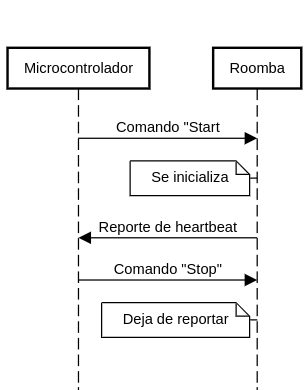
\includegraphics[scale=0.6]{./Figures/comm_test2.png}
    \caption{Diagrama de secuencias ejecutadas durante el test de comunicación entre el microcontrolador y el Roomba.}
    \label{fig:secMicroRoomba}
\end{figure}

\subsection{Validación de conexión bidireccional microcontrolador-ROS}

Descripción de la conexión con ROS usando un mensaje de "ping" con una doble confirmación. Pequeño diagrama explicando el método.

\begin{figure}[ht]
    \centering
    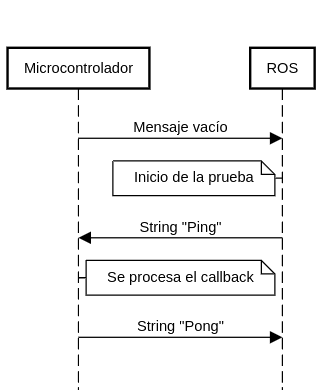
\includegraphics[scale=0.6]{./Figures/comm_test1.png}
    \caption{Diagrama de secuencias ejecutadas durante el test entre el microcontrolador y una PC con ROS.}
    \label{fig:secMicroROS}
\end{figure}

\subsection{Validación de frenado de emergencia}

El Roomba funciona de una manera tal que si este recibe un comando de velocidad, el mismo será aplicado al robot por un tiempo indefinido. De modo a prevenir riesgos, se implementó en el controlador un sistema de frenado de emergencia que responde a los siguientes pasos:

\begin{itemize}
    \item Se activa en cuanto se recibe un comando de velocidad distinto de cero.
    \item Se activa una tarea periódica, ejecutada cada 500 ms en donde se comprueba la existencia de al menos un mensaje nuevo en el tópico \file{/cmd\_vel}.
    \item En caso que no haya ningún mensaje, la tarea envía la orden de detener el robot.
\end{itemize}

\subsection{Validación de desplazamiento efectivo del robot}

El Roomba implementa su propio sistema de control interno para llevar sus ruedas hasta el \textit{set point} requerido por los comandos de velocdad. En visto que esta funcionalidad es crítica para el sistema, se desarrolló un caso de prueba especial consistente en lo siguiente:

\begin{itemize}
    \item mediante un script de Python conectado a ROS se envió un comando, el cual establece la velocidad de ambas ruedas a 0.1 m/s por una duración de 10 s es decir, el equivalente a un desplazamiento lineal de 1 m.
    \item mediante una cinta métrica se compararon los valores esperados con el desplazamiento lineal real.
    \item el mismo procedimiento se llevó a cabo con velocidad lineal negativa.
\end{itemize}

\begin{table}
    \centering
    \caption[Desplazamiento robot]{Resultados de validación de desplazamiento efectivo del robot}
    \begin{tabular}{lccc}
        \toprule
        \textbf{Movimiento} & \textbf{Desplazamiento} & \textbf{Desplazamiento} & \textbf{Error} \\
                            & \textbf{deseado}        & \textbf{obtenido}       &                \\
        \midrule
        Lineal positivo 1 m & 1 m                     & 0.97                    & 3 \%           \\
        Lineal negativo 1 m & -1 m                    & -0.91                   & 9~             \\
        \bottomrule
        \hline
    \end{tabular}
    \label{tab:desplazamientoRobot}
\end{table}

\subsection{Validación de lectura de encoders}

Dado que es posible obtener las lecturas crudas de los encoders del robot, se realizó la comprobación siguiente de manera similar a la prueba anterior:

\begin{itemize}
    \item mediante un script de Python conectado a ROS se envió un comando de velocidad, el cual establece la velocidad de ambas ruedas a 0.1 m/s por una duración de 10 s es decir, el equivalente a un desplazamiento de 1 m.
    \item mediante los encoders se obtuvo la cantidad de \textit{ticks} o cuentas ocurridas durante dicho periodo.
    \item se calculó el desplazamiento estimado mediante la fórmula $nTicks * 2 * PI * R / ticksPorVuelta$.
\end{itemize}

\subsection{Validación de lecturas crudas de IMU}

Esta prueba consistió en graficar las lecturas de los 6 ejes con respecto al tiempo respecto a cuatro movimientos generados de forma manual por el autor.

Para esta prueba se partió de un estado inicial con la IMU quieta, con el plano definido por sus ejes $(X,Y)$ en posición normal al vector de aceleración de la gravedad (que apunta al centro de la tierra).Para todas las pruebas se utilizó la convención de la mano derecha tanto para la definición de ejes ordenados como los sentidos de giro.

\begin{enumerate}
    \item Movimiento de aproximadamente 90 grados positivos alrededor del eje $Z$ y posterior retorno a la posición inicial.
    \item Movimiento de aproximadamente 90 grados positivos alrededor del eje $Y$ y posterior retorno a la posición inicial.
    \item Movimiento de aproximadamente 90 grados positivos alrededor del eje $X$. y posterior retorno a la posición inicial.
\end{enumerate}

En el gráfico del acelerómetro se puede apreciar el vector de aceleración de la gravedad apuntando en la dirección negativa del eje Z en su posición inicial.
% TODO
\begin{itemize}
    \item Durante el movimiento 1, el giroscopio mientras que el acelerómetro.
    \item Durante el movimiento 2, el giroscopio mientras que el acelerómetro.
    \item Durante el movimiento 2, el giroscopio mientras que el acelerómetro.
\end{itemize}

\section{Pruebas unitarias en la PC}

En esta sección se describen las pruebas realizadas sobre los resultados arrojados por los componentes de software ejecutados en una PC. Estos se utilizan para procesar los datos crudos arrojados por los sensores y generar información en un formato aprovechable por ROS.

\subsection{Validación de cálculo de odometría con encoders}

Esta prueba tuvo como objetivo validar el correcto funcionamiento del programa \file{lubo\_odom\_node}, el cual consume las lecturas de encoders y realiza con estas una estimación de la posición y orientación del robot en un plano $(X,Y)$.

Para la validación de esta característica se ejecutó la prueba descrita a continuación:

\begin{itemize}
    \item mediante un script de Python conectado a ROS se envió un comando de velocidad, el cual establece la velocidad de ambas ruedas a 0.1 m/s por una duración de 10 s es decir, el equivalente a un desplazamiento de 1 m.
    \item se realizó la
\end{itemize}

\subsection{Validación de estimador de pose con filtro Madwick para IMU}

El IMU MPU6050 no ofrece medición de campo magnético, por este motivo la información que provee resulta limitada e insuficiente para estimar la orientación absoluta del dispositivo.
Existen varias soluciones diferentes distintas para esta problemática pero para este trabajo se eligió utilizar un estimador de pose, es decir, un filtro especial que toma la información en bruto de acelerómetro y giroscopio y a su salida provee además de los valores filtrados de sus entradas, una estimación de la orientación del sensor.

Descripción de los resultados arrojados por la IMU MPU6050 en bruto. Gráfico de rqt\_plot
Resultados arrojados por las mismas mediciones, esta vez con el filtro activado.

\subsection{Validación de estimador de odometría con encoders + IMU}

Gracias a la aplicación de un Filtro de Kalman Extendido por parte del paquete \file{robot\_localization}, se combinó la información provista por el cálculo de odometría a partir de encoders con el estimador de pose proveniente de la IMU.

Esta pruebe consistió en comparar los valores de odometría arrojados por los encoders y por otro lado, la estimación de odometria resultante al combinar el primer valor con la pose de la IMU.

En la siguiente figura se puede apreciar el movimiento registrado por ambas fuentes de odometría para un desplazamiento lineal de 1 m, seguido de un giro de 90 grados para luego concluir con un segundo desplazamiento de 1m de modo a describir una figura en L en el plano $(X,Y)$.

\section{Pruebas de integración en campo}

En esta sección se describen las pruebas funcionales ejecutadas sobre cada uno de los módulos que componen el robot de manera aislada. Esto permitió encontrar problemas puntuales y reducir las fuentes de error para las pruebas de integración que le siguieron.

\subsection{Generación de mapa con gmapping}

Esta prueba consistió en la generación de un mapa del tipo \textit{occupancy grid} o mapa de ocupación, el cual consiste en una representación similar a la de un plano en dos dimensiones como los utilizados en arquitectura. Los puntos en negro representan una sección "ocupada" mientras que los píxeles blancos representan un área libre.

Para que el resultado obtenido a partir de este procedimiento sea lo suficientemente preciso como para ser usado para la posterior localización del robot fue necesario que la fuente de odometría sea muy precisa, motivo por el cual resultó necesario el uso de la fuente de odometría filtrada con información de la IMU. En las figuras se puede comparar el resultado obtenido a partir de las dos fuentes de odometría distintas.

%TODO: agregar imagenes de 1) Mapa horrible sin ekf 2) mapita decente con ekf.

\subsection{Localización en mapa con amcl}

Tal como se describió en la sección \ref{sec:amcl}, amcl es un paquete para ROS que provee al robot la capacidad de encontrar su posición y orientación de un mapa previamente provisto. Esta prueba consistió en la utilización de un mapa generado de la sala de estar del departamento del autor. Este fue provisto a la herramienta amcl mediante el servidor de parámetros de ROS y luego se procedió a teleoperar el robot mediante un \textit{joystick} inalámbrico.

La prueba se realizó de manera idéntica para tres puntos elegidos en el mapa. El procedimiento utilizado para cada uno de estos puntos fue el siguiente:

\begin{enumerate}
    \item por medio del \textit{joystick} se hizo girar al robot en círculos en sentido horario hasta completar dos vueltas completas de 360 grados a una velocidad angular aproximada de 0,5 rad/s.
    \item se aplicó el mismo procedimiento para un giro en sentido anti-horario.
    \item se guardó una captura de pantalla de la localización del robot en RViz.
\end{enumerate}

% TODO: Agregar los tres screenshots

\subsection{Navegación en mapa con move\_base}

Así como se describe en la sección \ref{sec:move_base}, move\_base provee la funcionalidad necesaria para mover un robot en un mapa provisto, para lo cual la herramienta se encarga de calcular una ruta de navegación desde el punto en que el robot se encuentra al momento de enviarse la orden y otro punto cualquiera del mapa.

Esta prueba consistió en indicar a la herramienta que deseabamos mover el robot de un punto a otro en el mapa. Para el envío puntos
Para que esta prueba pueda realizarse fue necesario cumplir con ciertos requisitos previos:

\begin{enumerate}
    \item un mapa estático debió ser provisto al servidor de mapas de ROS.
    \item el robot debió encontrarse previamente localizado en el mapa.
\end{enumerate}
